\section{Продвинутые подходы автоматизации тестирования} 

До настоящего момента под <<автоматизацией>> понималась автоматизация выполнения тестов. Продвинутые подходы к автоматизации тестирования расширяют понятие атоматизиции. Они исключают человеческий фактор в процессе тестирования. Это означает отсутсвие необходимости разрабатывать тестовые сценарии. Компьютер сделает это за человека. Иногда такие подходы называются тестированием с помощью искусственного интелекта.

\subsection{Статическое тестирование} 

Статическое тестирование (статический анализ)~--- автоматизированный процесс ревизии кода без его исполнения. Статическое тестирование позволяет быстро найти ошибки низкой и средней сложности (использование неактуальной библиотеки, обращение к пустому указателю и т.~д.). Распространенные инструменты статического анализа: \textit{PMD, Checkstyle, Checkmarx}.

Классический подход к статическому анализу заключается в проверке исходного кода системы на потенциальные структурные или стилистические уязвимости. Анализатор состоит из парсера и набора правил. Существуют две техники статического анализа:


\begin{enumerate}
	\item Сопоставление с образцом с помощью регулярных выражений.
	\item Синтаксический анализ абстрактного ситаксического дерева.
\end{enumerate}


\subsubsection{Сопоставление с образцом}

Сопоставление с образцом~--- проверка кода, входе которой происходит поиск соответствия заданному ранее образцу. Образец задается с помощью \textbf{регулярного выражения}. Регулярное выражение~--- последовательность символов, представляющая образец.

Недостатком сопоставления с образцом является отсутствие контекста исполнения. Другими словами, сопоставление с образцом не учитывает семантику программы. Например, задав регулярное выражение \texttt{$\textbackslash$s*System.out.println\textbackslash(.*\textbackslash);} сопоставление с образцом определит 3 строки в листинге~1.17. Из чего можно сделать вывод, что программа напечатает 3 раза некоторое сообщение. Однако, программа не напечатает ни одного сообщения. 

\begin{ListingEnv}[!h]% настройки floating аналогичны окружению figure
	\captiondelim{ } % разделитель идентификатора с номером от наименования
	\caption{Пример неучитанной семантики}
	% окружение учитывает пробелы и табуляции и применяет их в сответсвии с настройками
	\begin{lstlisting}[language={Java}]
boolean DEBUG = false;

if (DEBUG){
	System.out.println("Debug line 1");
	System.out.println("Debug line 2");
	System.out.println("Debug line 3");
}
	\end{lstlisting}
\end{ListingEnv}%


\subsubsection{Синтаксический анализ}

Более продвинутый способ анализа кода~--- синтаксический анализ. В ходе синтаксического анализа текст программы разбивается на поток символов, символы пребразубтся в токены, а из токенов составляется \textit{дерево разбора}. Дераво разбора представляет собой синтаксическое дерево конкретной версии кода. В синтаксическом анализе используется \textit{абстрактое синтаксическое дерево}~--- дерево разбора без синтаксических деталей (точки с запятой, скобки). Пример абстрактного синтаксического дерева кода из листинга~1.17 представлен на рис.~\ref{img:ast}

\begin{figure}[ht]
	\centering
	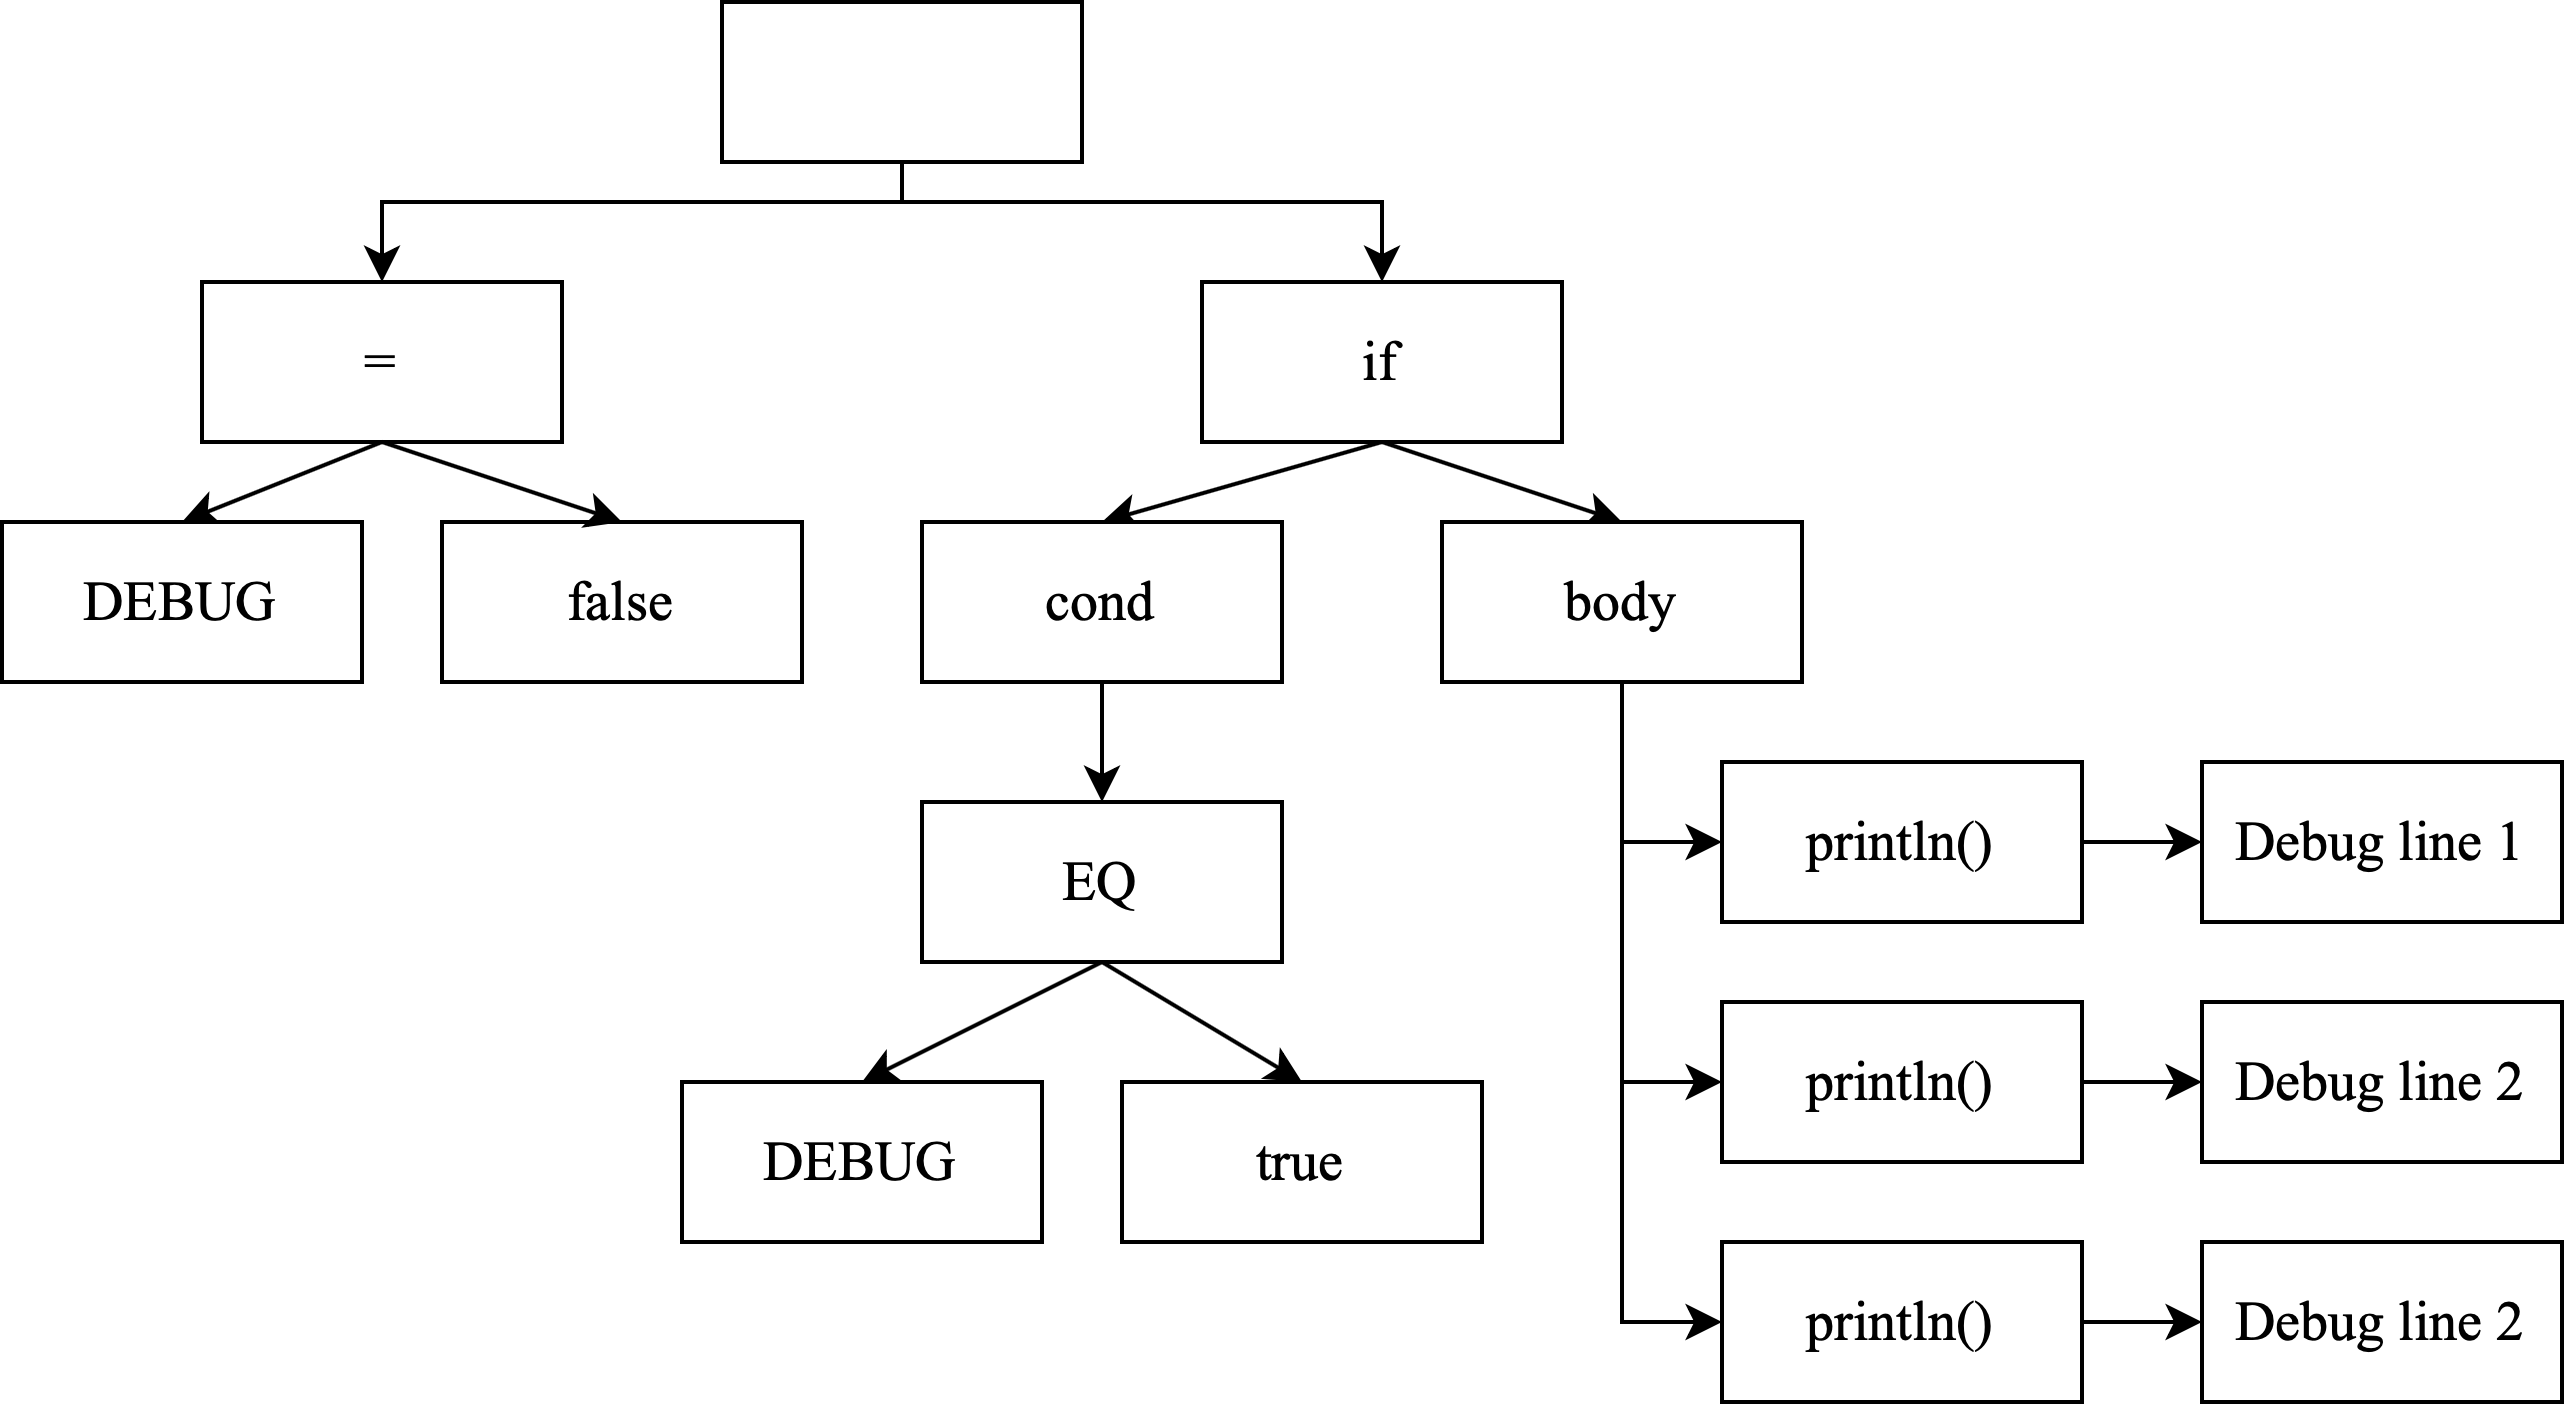
\includegraphics [scale=0.9] {AST_TR}
	\caption{Абстрактное синтаксическое дерево}
	\label{img:ast}
\end{figure}


Статический анализатор, использующий ситаксический анализ, принимает на вход абстрактное синтаксическое дерево и набор правил. Анализатор сообщает о найденных несоответствиях в коде.


\subsection{Мутационное тестирование} 
  
При рассмотрении структурного тестирования были описанны различные критерии покрытия кода. Эти критерии нужны для того, чтобы измерить объем кода, выполненного в ходе тестирования. К сожалению, таких критериев может быть не достаточно для оценки качества тестов. Например, тест может достигать 100~\% покрытия кода, но в то же время не содержать проверок (assertions). То есть тест запускает код, но не тестирует результат его исполнения. Мутационное тестирование решает эту проблему.
 
Критерий, который отражает насколько эффективнен тест, называется критерием \textit{способности определения ошибок(fault detection capability)}. Этот критерий составляет основу \textbf{мутационного тестирования}. В процессе мутационного тестироания в код программы добавляются (искуственно) ошибки. После чего запускается набор тестов и проверяется, смогли ли тесты найти ошибку. Цель мутационного тестирования~--- повышение качества тестирующего кода. Чем больше ошибок тест может найти, тем выше его эффективность.

Терминология в мутационном тестировании:

\begin{itemize}
	\item \textbf{Мутант.} Для данной программы \textit{P}, мутантом называется программа \textit{P'}, полученная из программы \textit{P} путём \textit{синтаксической трансформации}. Мутант считается убитым, если он не проходит хотя бы один тест.
	\item \textbf{Синтаксическая трансформация.} Небольшое изменение кода, при котором код все еще компилируется.
	\item \textbf{Изменение.} Имитация типичной человеческой ошибки. 
\end{itemize}

Для атоматизации мутационного тестирования необходимо определить \textbf{мутационный оператор}. Мутационный оператор~--- граматическое правило, которое может быть использования для создания синтаксической трансформации. Например, замена знака \(+\) на 
\(-\) в арифметических выражениях. Распространенные мутационные операторы:

\begin{itemize}
	\item \textbf{Оператор арифметической замены.} Замена арифметечиского оператора на другой. Арифметические операторы: \texttt{+, -, *, /,\%}.
	\item \textbf{Оператор замены сравнений.} Замена операторов \texttt{<=, >=, !=, ==, >, <}.
	\item \textbf{Оператор логической замены.} Замена операторов \texttt{\&\&, ||, \&, |, !, \^}.
	\item \textbf{Оператор замены присваения.} Замена операторов \texttt{=, +=, -=, /=}.
	\item \textbf{Оператор замены скалярных переменных.}  Замена одной переменной на другую.
\end{itemize}

Помимо описанных выше метационных оперторов, существуют операторы, ориентированные на особонности языка. Например, оператор замены модификоторов видимости, переопределение метода и т.~д.

Для оценки качества тестового сценария с помощью мутационного анализа используется \textit{критерий устойчивости к мутациям}.

\[ \text{критерий устойчивости к мутациям} = \frac{\text{количество убитых мутантов}}{\text{общее количество мутантов}}  \]

Чем больше мутантов убивает тест, тем выше его критерий устойчивости к мутациям. Соответсвенно, этот тест найдет больше реальных ошибок программистов. 

Недостатком мутационного тестирования является время исполнения. На проектах средней сложности (300 файлов) мутационное тестирование занимает около 10 минут~[9].

В языке Java для мутационного тестирования используется инструмент PIT~[10].

\subsection{Генерация псевдосдослучайных входных данных} 
 
Генерация псевдосдослучайных входных данных или фаззинг (англ. Fuzzing)~--- техника тестирования программного обеспечения, основанная на автомаческой генерации псевдослучайных входных данных~[11]. Цель фаззинга~--- поиск \textit{ошибок, утечек памяти, неудачных обработок ошибок и уязвимостей безопастности}.

Существует несколько способов генерации входных данных:

\begin{itemize}
	\item \textbf{Случайная генерация.} Тестируемая система принимается за черный ящик, предположений о формате входных данных не делается. Генерируется большое количество случайных данных и подается на вход программе. На практике этот способ редко используется. Для построения более эффективных фаззеров испольщуется \textit{структурированные входные данные}, которые предопределенны.
	\item \textbf{Мутирующие фаззеры.} На вход фаззеру даётся пример входных данных. Фаззер применяет различные мутации к данным и проверяет поведение системы. Примеры мутаций: замена символов в строке, замена битов. Некоторые инструменты (American Fuzzy Lop) используют генетические алгоритмы для повышения качества входных данных.
	\item \textbf{Генеративные фаззеры.} Генеративные фаззери или \textit{протокольные фаззеры} принимают на вход формат входных данных. Например, если программа обрабатывает файлы в формате \texttt{jpeg}, то генеративный фаззер будет генерировать файлы только формата \texttt{jpeg}.
\end{itemize}
 
 Мутирующие фаззеры более гибкие и проще в использовании, чем генеративные. Но генеративные фаззеры достигают большего покрытия кода и производят более эффективные тестовые сценарии.
 
 Генерация случайных данных~--- затратный процесс с точки зрения процессорного времени. Для оптимизации это процесса используется    \textit{техники сокращения времени генерации.}
 
 
 \subsubsection{Использование нескольких фаззеров}
 
 Самый простой способ увеличить покрытие кода~--- использование нескольких фаззеров одновременно. Каждый фаззер генерирует входные данные по собственному алгоритму. Это приводит к повышению качества тестовых сценариев и сокращению общего времени генерации (100~\% покрытия достигается быстрее).
 
 \subsubsection{Использование телеметрии кода}
 
 Телеметрия кода (данные о покрытии) может быть полезна для коррекции стратегии генерации. Например, фаззер может использовать только тот набор входных данных, который повышает показатель покрытия кода и отбросить большую часть сгенерированных данных.
  
 \subsubsection{Символическое исполнение}
 
 Для определения набора входных параметров, необходимых для достижения определенного участка кода, используется символическое исполнение. Можно составить формулу для определенного пути, которая отвечает на вопрос: существует ли такой набор данных, который приводит к исполнению определенной строки кода? Если да, то какой. 
 
\textit{Z3} является самым популярным инструментом для символического исполнения. На вход он получает участки кода, которые нужно достичь. Результатом работы является набор ограничений для входных данных, которые должны выполняться, чтобы достичь определенных участков кода. Результат работы \textit{Z3} учитывается генеративным или мутационным фаззером с целью оптимального подбора входных параметров. 

В листинге~1.18 определяется функция с двумя входными параметрами a и b. Для удовлетворения предиката \texttt{else if} нужно удовлетворить ограничениям \(((N + M <= 2)\&(N < 100))\). Ограничение выводится следующим образом:

\begin{enumerate}
	\item \texttt{a} и \texttt{b} преобразуются в символы  \(a = N, b = M\).
	\item Операторы присвоения трансформируют \texttt{a} и \texttt{b} в  \(a = N + M, b = (N + M) - M = N\).
	\item Ограничение оператора \texttt{if}: \((N + M > 2)\), для остальных веток исполнения это \(N + M <= 2\).
	\item Ограничение ветки \texttt{else if}: \(N < 100\).
	\item Итоговое ограничение ветки \texttt{else if} является комбинацией  двух предыдущих:  \( (N + M <= 2) \& (N < 100)\)
\end{enumerate}

\begin{ListingEnv}[!h]% настройки floating аналогичны окружению figure
	\captiondelim{ } % разделитель идентификатора с номером от наименования
	\caption{Пример кода}
	% окружение учитывает пробелы и табуляции и применяет их в сответсвии с настройками
	\begin{lstlisting}[language={Java}]
public String func(int a, int b){
	a = a + b;
	b = a - b;
	String str = "No";
	if (a > 2)
		str = "Yes!";
	else if (b < 100)
		str = "Maybe!";
	return str;
}
	\end{lstlisting}
\end{ListingEnv}%

Стоит отметить, что не всегда код является разрешимим с точки зрения символического исполнения.


\subsection{Тестирование на основе анализа кода} 
 
 Тестирование на основе анализа кода (англ. Search-based software testing,  SBST)~--- автоматизированный процесс анализа исходного кода и генерации для него тестовых сценариев. 
 
 Основаня цель SBST~--- достижение 100~\% покрытия кода минимальным набором тестов. Это задача оптимизации~[12,13]. Прежде чем рассмотреть, как она решается, нужно понять как работают инструменты  анализа и генерации кода. Для класса из листинга~1.19 алгоритм генерации тестов будет выглядеть следующим образом: 
 
 \begin{enumerate}
 	\item Создать экземпляр класса.
 	\item Если конструктор имеет параметры, сгенерировать случайные параметры и подставить их.
 	\item Вызвать тестируемый метод.
 	\item Если метод имеет параметры, сгенерировать их случайным образом и подставить.
 	\item Если метод вернул релультат, сохранить его в переменную.
 	\item Использовать полученный результат для написания утверждений (assertions).
 	\item Замерить полученное покрытие кода.
 	\item Повторить все действия, пока не будет достигнуто суммарное покрытие тестами 100~\% или закончится время.
 \end{enumerate}

\begin{ListingEnv}[!h]% настройки floating аналогичны окружению figure
	\captiondelim{ } % разделитель идентификатора с номером от наименования
	\caption{Пример кода, определяющего тип треугольника}
	% окружение учитывает пробелы и табуляции и применяет их в сответсвии с настройками
	\begin{lstlisting}[language={Java}]
public class Triangle {
	
	private final int a, b, c;
	
	enum TriangleType {
		EQUILATERAL, ISOSCELES, SCALENE
	}
	
	public Triangle(int a, int b, int c) {
		this.a = a;
		this.b = b;
		this.c = c;
	}
	
	public TriangleType classify(int a, int b, int c) {
		if (a == b && b == c)
			return TriangleType.EQUILATERAL;
		else if (a == b || b == c)
			return TriangleType.ISOSCELES;
		else
		return TriangleType.SCALENE;
	}
}
	\end{lstlisting}
\end{ListingEnv}%


Пример случайно сгенерированного тестового сценария представлен в листинге~1.20.

\begin{ListingEnv}[!h]% настройки floating аналогичны окружению figure
	\captiondelim{ } % разделитель идентификатора с номером от наименования
	\caption{Случайно сгенерированный тест}
	% окружение учитывает пробелы и табуляции и применяет их в сответсвии с настройками
	\begin{lstlisting}[language={Java}]
@Test
void t1() {
	Triangle t = new Triangle(5, 7, 10);
	Triangle.TriangleType type = t.classify();
	assertThat(type).isEqualTo(Triangle.TriangleType.SCALENE);
}
	\end{lstlisting}
\end{ListingEnv}%

Для оптимизации времени генерации и качества тестовых сценариев используется ряд эвристик. Самый популярный способ оптимизации~--- генетический алгоритм. Фунцией оптимизации является критерий покрытия. Чем он выше, тем больше шансов у определенного теста пройти этап селекции и попасть в итоговый набор тестов. Критерий покрытия может быть разный. Самый распространенный~--- критерий покрытия веток исполнения. 

Тестирование на основе анализа кода~--- область компьютерных наук, которая находится в стадии активного изучения. На данный момент не существует широко распространненых инструментов автоматической генерации тестов. В научных сообществах есть два инструмента: Randoop~[14] и Evosuite~[15]. Существует платный инструмент Cover, разработанный компанией Diffblue, которая занимается разработкой программных продуктов для анализа кода~[16].  Одну из певых попыток использовать SBST в промышленной разработке стала компания Facebook со своим инструментом Sapienz~[17] для автоматической генерации тестовых сценариев для мобильного приложения. 

